
\documentclass[]{interact}

\usepackage{epstopdf}% To incorporate .eps illustrations using PDFLaTeX, etc.
\usepackage[caption=false]{subfig}% Support for small, `sub' figures and tables
%\usepackage[nolists,tablesfirst]{endfloat}% To `separate' figures and tables from text if required
%\usepackage[doublespacing]{setspace}% To produce a `double spaced' document if required
%\setlength\parindent{24pt}% To increase paragraph indentation when line spacing is doubled

% \usepackage[longnamesfirst,sort]{natbib}% Citation support using natbib.sty
% \bibpunct[, ]{(}{)}{;}{a}{,}{,}% Citation support using natbib.sty
% \renewcommand\bibfont{\fontsize{10}{12}\selectfont}% To set the list of references in 10 point font using natbib.sty

\usepackage[natbibapa,nodoi]{apacite}
\setlength\bibhang{12pt}
\renewcommand\bibliographytypesize{\fontsize{10}{12}\selectfont}

\usepackage{xcolor}

%\usepackage[natbibapa,nodoi]{apacite}% Citation support using apacite.sty. Commands using natbib.sty MUST be deactivated first!
%\setlength\bibhang{12pt}% To set the indentation in the list of references using apacite.sty. Commands using natbib.sty MUST be deactivated first!
%\renewcommand\bibliographytypesize{\fontsize{10}{12}\selectfont}% To set the list of references in 10 point font using apacite.sty. Commands using natbib.sty MUST be deactivated first!

\theoremstyle{plain}% Theorem-like structures provided by amsthm.sty
\newtheorem{theorem}{Theorem}[section]
\newtheorem{lemma}[theorem]{Lemma}
\newtheorem{corollary}[theorem]{Corollary}
\newtheorem{proposition}[theorem]{Proposition}

\theoremstyle{definition}
\newtheorem{definition}[theorem]{Definition}
\newtheorem{example}[theorem]{Example}

\theoremstyle{remark}
\newtheorem{remark}{Remark}
\newtheorem{notation}{Notation}

\begin{document}

%\articletype{ARTICLE TEMPLATE}% Specify the article type or omit as appropriate
\title{Deep Reinforcement Learning for Navigation of Mobile Robots}

\author{
\name{Junior C. Jesus\textsuperscript{a}\thanks{Email: dranaju@gmail.com (Junior C. Jesus)}, Jair A. Bottega\textsuperscript{a}\thanks{Email: jairaugustobottega@gmail.com (Jair A. Bottega)} and Daniel F. T. Gamarra\textsuperscript{a}\thanks{Email: daniel.gamarra@ufsm.br (Daniel F. T. Gamarra)}}
\affil{\textsuperscript{a}Federal University of Santa Maria, Santa Maria, RS, Brazil}
}

\maketitle

\begin{abstract}
This paper presents a study of a deep reinforcement learning technique that uses a Deep Deterministic Policy Gradients network for application in navigation of mobile robots.
In order for the robot to arrive to a target on a map, the network has 10 laser range findings, the previous linear and angular velocity, and relative position and angle of the mobile robot to the target as inputs. As outputs, the network has the linear and angular velocity.
From the results analysis, it is possible to conclude that the deep reinforcement learning’s algorithms, with continuous actions, are effective for decision-make of a robotic vehicle. 
However, it is necessary to create a good reward system for the intelligent agent to accomplish your objectives.
This research uses different virtual simulation environments provided by ROBOTIS in the robot simulation software Gazebo in order to test the performance of the algorithm.
\end{abstract}

\begin{keywords}
Deep Deterministic Policy Gradients, Deep Reinforcement Learning, Robot’s Navigation.
\end{keywords}

\section*{Introduction}
Deep Reinforcement Learning (Deep-RL) is starting to achieve interesting results in different areas such as tasks involving the control on discrete systems \citep{mnih2013playing}, \citep{schaul2015prioritized} continuous systems \cite{lillicrap2015continuous}, \cite{schulman2015high}, %\cite{nachum2017trust}
and more recently in robotics \cite{gu2017deep}, \cite{mahmood2018benchmarking}.
The first applications of deep reinforcement learning in robotics were in the use of manipulation in a  fully observable and stable environment \cite{gu2016continuous}, but tasks in mobile robotics involving obstacles interacting with physical environments and objects, turns the workplace more complex.
In order to overcome this problem, Deep-RL methods normally try to discretize the actions to turn simpler the problem \cite{zhu2017target}, \cite{tai2016towards}.
Recent articles explore continuous control actions used for navigation of mobile robots with good results \cite{tai2017virtual}, \cite{chen2017socially}.

In this paper, we try to demonstrate how effective can be the Deep-RL used on simulated environments.
For that, three environments were used on Gazebo, which can provide us with a lot of resources for robot simulation, for example we can create an environment and insert a model of a real mobile robot \cite{fairchild2016ros}, \cite{joseph2015mastering}. 
The mobile robot used on the simulation was the TurtleBot3.

The objective of this research is to show the efficiency of a Deep-RL network in the task of mobile robot navigation from an initial position to a target on an environment.
To simplify this problem it was created a network which has 14 inputs and 2 outputs, as shown in Fig. \ref{fig:mapless}.
The 14 inputs are composed by 10 readings of the laser sensor, the previous linear and angular velocity, the distance and angle of the mobile robot related to the target.
And the outputs of the network are the linear and angular velocity that are sent to the robot in order to get to the target.
It is expected the intelligent agent won't collide with any obstacle on its trajectory to the target.

\begin{figure}[H]
\centerline{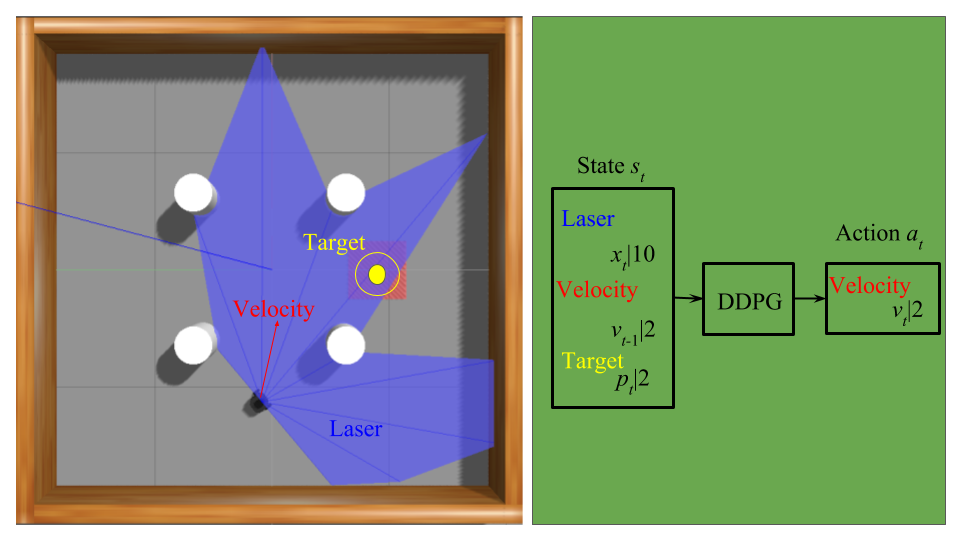
\includegraphics[width=12cm]{images/mapless_en.png}}
\caption{System definition.}
\label{fig:mapless}
\end{figure}

This work is divided in seven sections.
After a brief introduction in the first section of the Deep-RL on the mobile robot navigation, the second section describes the work of authors on the field that inspired this research, the third section gives a background about the technique used, the fourth section makes an introduction of the tools used for the project, the fifth section summarizes the methods so that the robot can get to a target, the sixth section presents the results obtained on the Gazebo environments, the seventh section makes the discussion on the results and applications of Deep-RL.

\section*{Related Works}

Deep-RL has been previously applied on robotic tasks, among these applications we can refer to the work of (Kober, Bagnell, and Peters \citeyear{kober2013reinforcement}; Stone, Sutton, and Kuhlmann \citeyear{stone2005reinforcement}; Tobin et al. \citeyear{tobin2017domain}).
Which is a survey of different works of these techniques applied to robotics.
Mnih et al. (Mnih et al. \citeyear{mnih2013playing}) utilized a convolution neural network to estimate a value function for future rewards on the Atari games, this strategy was called deep Q-network (DQN)(Mnih et al. \citeyear{mnih2013playing}; Hausknecht and Stone \citeyear{hausknecht2015deep}; Van Hasselt, Guez, and Silver \citeyear{van2016deep}).
The DQN can only be used in a task with a discrete action.
To extend it to a continuous control, Lillicrap et al. (Lillicrap et al. \citeyear{lillicrap2015continuous}) proposed a deep deterministic policy gradients (DDPG).
That became the basement for the application of Deep-RL in mobile robot navigation.
Tai et al. (Tai et al. \citeyear{tai2017virtual}) created a mapless motion planner for a mobile robot by taking the sparse 10-dimensional range findings and the target position with respect to the mobile robot coordinate frame as inputs and the continuous steering commands as output, but firstly being proposed as discrete steering commands on (Tai and Liu \citeyear{tai2016towards}). It was shown that, with the asynchronous Deep-RL method, a mapless motion planner can be trained and complete the task to get to a determined target. 

Zhu et al. (Zhu et al.\citeyear{zhu2017target}) proposed another model to apply the Deep-RL to the task of driving a mobile robot.
The model created took the current observation of states and the image of the target as input and generated an action in a 3D environment as the output.

An activity that can be very challenging in robotics is to navigate a vehicle safely and efficiently in pedestrian-rich environments. Chen et al. (Chen et al. \citeyear{chen2017socially}) elaborated a Deep-RL model that can quantify what \textit{to} do and \textit{not to} do on the precise mechanism of human  navigation.
This work develops a time-efficient navigation policy that respects common social norms.
Creating a method able to control a mobile robot moving at human walking speed in an environment with many pedestrians.

\section{Theoretical Background}


\subsection{Deep Reinforcement Learning}

The goal in deep reinforcement learning is to control an agent attempting to maximize a reward function. 
The deep Q-network (DQN) algorithm \cite{mnih2013playing} was capable of human level performance on many Atari video games by estimating the actions of an agent.
However, while DQN could solve problems on complex observation spaces, it only can handle discrete action spaces. 
It is noticeable that many tasks, on the robotic control, have continuous action spaces. 
So DQN cannot be applied to continuous domains and it is necessary to use another algorithm that can handle this type of problems.

The deep deterministic policy gradients (DDPG) algorithm consists of an actor-critic method that uses approximation functions that can learn continuous action space policies. The algorithm makes use of a neural network for the actor network and other for the critic network. These two networks computes the action prediction  for the current state and generates a temporal-difference error signal for each time step. The input of the actor network is the current state, and the output is a real value representing an action chosen for a continuous action space. The output of the critic is simply the estimated Q-value of the current state and the action given by the actor.

The biggest challenge of learning in continuous action space is exploration.
To confront this challenge is needed to construct a exploration policy $\mu'$ by adding a noise sampled from a noise process $\mathcal{N}$ to the actor network policy, defined as:
\begin{equation}
\mu' = \mu(s_t) + \mathcal{N}
\end{equation}
where $\mathcal{N}$ can be chosen in a way to suit the environment.
Being the Ornstein-Uhlenbeck process \cite{uhlenbeck1930theory} the most used to generate temporally correlated exploration efficiency in physical control problems.

In general, to train and evaluate a policy function coming out of the actor network and a value function coming out of the critic network, with thousands of simulated trajectories temporally correlated, leads to the introduction of huge amounts of variance in the approximation of a true Q-function.
It is suggested to use a replay memory to store the experiences of the agent during training \cite{schaul2015prioritized}.
This means, saving the states, actions, rewards and new states that the agent explored during the episode.
And then, randomly sampling experiences to use  for learning in order to break the temporal correlations within different training episodes.

The replay of experiences allows the intelligent agent to learn from recent memories, increasing  the learning speed and breaking undesirable temporal correlations.
Even with a short memory it is possible to see a substantial improvement in the agent performance.
Despite the application of a replay memory slows the agent learning, a better performance is achieved.

Without counting the replay memory used, it is needed to make a target network to generate targets for the temporal-difference error that can regulate the learning and improve stability.
The target network contains a copy of the actor and critic, however, with ``soft" updates.
This means that the target network do not copy directly the weights of the actor and critic network.
The weights, represented by $\theta$, of the target network are then updated by:
\begin{equation}
    \theta' \leftarrow \tau\theta + (1-\tau)\theta
\end{equation}
with $\tau \ll 1$. 
Where the target is represented by the apostrophe.
So the target values of the network change slowly and allows an improvement in the stability of the learning.


\section*{Experimental Setup}

For the analysis of a DDPG network was used the programming language Python \cite{ascher1999learning}. 
The Python language has as priority the legibility of the code under speed. 
The vast library and frameworks provided by Python makes it an exquisite tool for machine learning and data analysis purposes.

\subsection*{ROS}

The robot operations system (ROS) is a flexible framework to write software for robots.
ROS \cite{pyo2015ros} is a collection of tools, and libraries.
ROS provides operational system's standard services, like hardware's abstraction, device low level control, messages between processes and package management. 
The set of ROS processes in execution are represented by graphs architecture where the processing is performed on nodes that receive and send messages as sensors, control, state, planning, actuator and others.

Despite the importance of low latency on the robots control, ROS is not a real-time operational system, although it is possible to integrate ROS with real-time code. This lack of real-time system is being addressed on the development of ROS 2.0.

\subsection*{TurtleBot}

TurtleBot is a ROS standard platform robot, and there are 3 version of the series. TurtleBots are affordable and programmable mobile robots for use in education, research, hobby, and product prototyping.
The third version was used on this project, shown in Fig. \ref{fig:turtlebot3}.

\begin{figure}[H]
\centerline{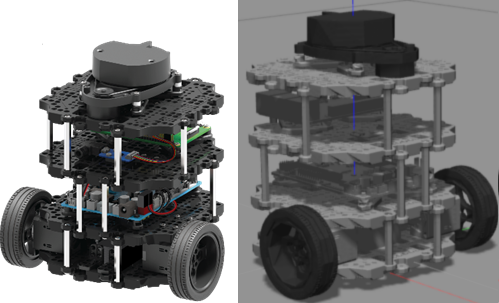
\includegraphics[width=12cm]{images/burger.png}}
\caption{Real and simulated TurtleBot3 Burger in Gazebo.}
\label{fig:turtlebot3}
\end{figure}

The TurtleBot3 Burger uses 2 DYNAMIXEL motord series XL, for the object detection the TurtleBot3 utilize a 360 degree sensor laser LiDAR, and it has an IMU sensor for the odometry calculations.
All the control is made by the open source controller board OpenCR1.0 and Raspberry Pi 3 microprocessor.
The Table \ref{tab1} shows all hardware specification of the TurtleBot3 version Burger.


\begin{table}[H]
\caption{Hardware Specification of the TurtleBot3 Burger}
\begin{center}
\begin{tabular}{|l|l|}
\hline
\textbf{Items}&\textbf{Specification} \\
\hline
Maximum translational velocity & 0.22 m/s \\
\hline
Maximum rotational velocity    & 2.84 rad/s (162.72 deg/s) \\
\hline
Maximum payload                & 15kg \\ 
\hline
Size (L x W x H)               & 138mm x 178mm x 192mm \\
\hline
Weight                         & 1kg \\
\hline
Threshold of climbing          & 10 mm or lower \\
\hline
Expected operating time        & 2h 30m \\
\hline
Expected charging time         & 2h 30m \\
\hline
SBC (Single Board Computers)   & Raspberry Pi 3 Model B and B+ \\
\hline
Actuator                       & DYNAMIXEL XL430-W250 \\
\hline
LDS(Laser Distance Sensor)     & 360 Laser Distance Sensor LDS-01 \\
\hline
IMU                            & \begin{tabular}[c]{@{}c@{}}Gyroscope 3 Axis\\ Accelerometer 3 Axis\\ Magnetometer 3 Axis\end{tabular} \\
\hline
Battery                        & \begin{tabular}[c]{@{}c@{}}Lithium polymer \\ 11.1V 1800mAh / 19.98Wh 5C \\ \end{tabular} \\
\hline

\end{tabular}
\label{tab1}
\end{center}
\end{table}

\subsection*{Gazebo}

Robot simulation is an essential tool on all roboticist's toolbox.
A good simulator makes possible to test algorithms quickly, to design robots, and to train systems with artificial intelligence using realistic scenarios.
With Gazebo \cite{fairchild2016ros} is possible to simulate this environments easily and with the advantage of having an active community.
This makes Gazebo a great tool on the area of robotic simulation.

\subsection*{OpenCV}

Open Source Computer Vision (OpenCV) is an open source computer vision and machine learning software library.
It is mainly used for developing advanced image processing and computer vision applications \cite{bradski2008learning}.
With OpenCV is possible to take frames out of a video and run algorithms to get necessary information.
It can be great to identify an object, recognize a face or track the movement of an object, extracting coordinates, for example, what is very useful and commonly used in the wide area of robotics.


\section*{Methodology}

The intention of this work is to create a mobile robot that can plan its movements without any map knowledge on the environment. Its translation function is defined as:
\begin{equation}
v_t = f(x_t, p_t, v_{t-1})
\end{equation}
where $x_t$ is the observation from the raw sensor information, $p_t$ is the relative position of the target, and $v_{t-1}$ is the velocity of the mobile robot in the last time step.
All variables specified, previously, can be defined as the current state $s_t$ of the mobile robot.
With this model it is possible to get the actions that the robot will make, given its current state.
However, it is needed to ensure a minimum reading frequency of the input data to control the movement of the robot because if the robot get a slow read frequency of the inputs it cannot react to an obstacle in the trajectory to a target. In this way, the robot can react to new states quickly.
This methods was first explored by Tai \textit{et al.} \cite{tai2017virtual}.

\subsection*{Network Structure}

Once the system of state and actions has been defined, it is possible to create a DDPG network capable of resolving the problem.
The DDPG network has 14 inputs as presented in Fig. \ref{fig:entradaESaida}, in which 10 corresponds to the laser range findings, 2 corresponds to the linear and angular velocity, and the other 2 corresponds to the relative position and angle of the mobile robot to the target.
The sample of the laser range findings are between $-90$ and $90$ degrees in relation to the robot. The output of the network is the action of linear and angular velocity that will be applied on the mobile robot.

\begin{figure}[H]
\centerline{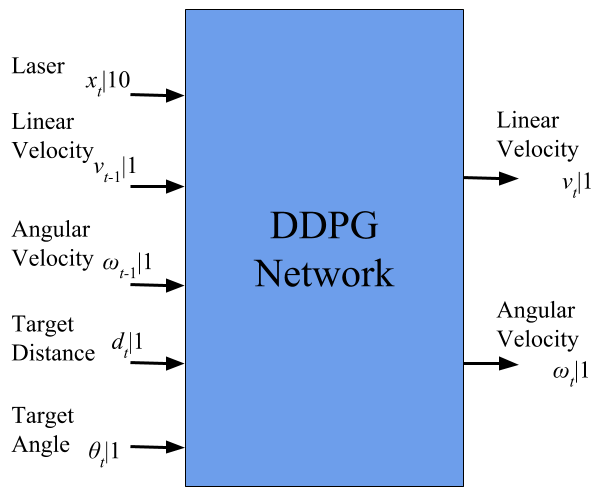
\includegraphics[width=8cm]{images/o_and_i.png}}
\caption{DDPG network inputs and outputs.}
\label{fig:entradaESaida}
\end{figure}

The network structure of the DDPG is shown in Fig \ref{fig:projetointegrador}. 
The actor-network has as input the current state of the mobile robot followed by 3 fully-connected neural networks layers with 512 nodes.
This input of the networks is transformed on the linear and angular velocity that will be the commands sent to the motor of the mobile robot. 
The angular velocity range is constrained between $(-1,1)$ and the hyperbolic tangent function $(tanh)$ is used as activation function.
For the linear angular range, that it is constrained between $(0,1)$, the sigmoid function was used.
As there is no laser readings in the back of robot, the backward move is not necessary.
The output actions are then multiplied with two hyperparameters to decide the final linear and angular velocity executed by the mobile robot.
For this, it was used as maximum linear velocity $0.22$ $m/s$ and maximum angular velocity $2$ $rad/s$ on the TurtleBot3 robot version Burger.


\begin{figure}[H]
\centerline{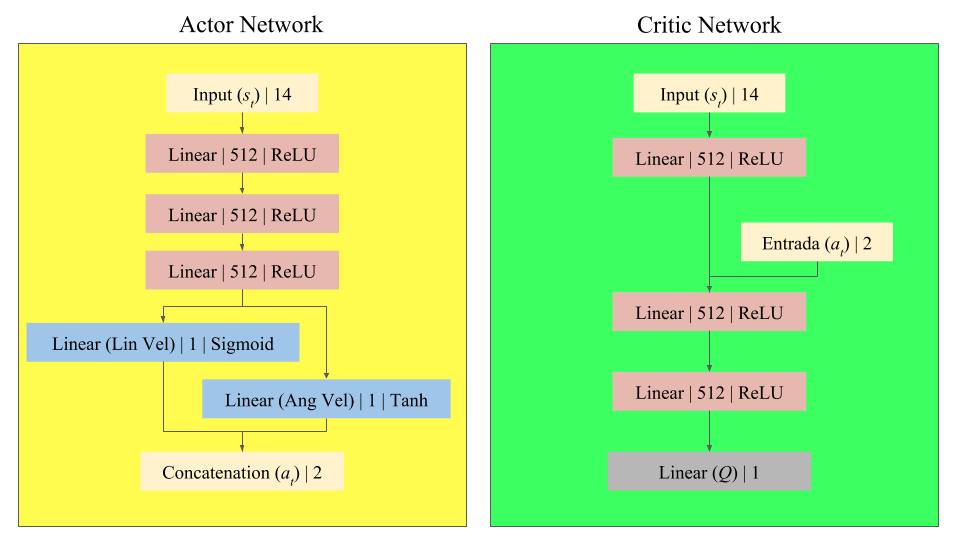
\includegraphics[width=12cm]{images/projeto_integrador_en.png}}
\caption{DDPG network structure model.}
\label{fig:projetointegrador}
\end{figure}

In the critic-network, the Q-value of the current state and action are predicted.
Using only 3 fully-connected neural networks layers to process the input state.
Where the action, output of the actor-networks, is concatenated on the second neural network layer.
The Q-value is activated through a linear activation function:
\begin{equation}
y = kx +b
\end{equation}
where $x$ is the input of the last layer, $y$ is the predicted Q-value, and $k$ and $b$ are the trained weights and bias of this layer, respectively.

\subsection*{Simulation Environments}

There were used three environments for the simulations. The first environment is  shown in Fig. \ref{fig:environments}(a), the environment represents a free area for the robot to move.
The walls of this environment are the only things where the robot can collide.
If the mobile robot collide with the wall or any obstacle, a negative reward is given for this action and the current episode stops.
The second environment is shown in Fig. \ref{fig:environments}(b) and has 4 fixed obstacles.
It means that this environment is more complex in a way that the intelligent agent have to make a better strategy to not collide.
The third environment, shown in Fig. \ref{fig:environments}(c), is more complex than the previous environments.  
The number of walls and the mobile obstacles, represented by the white blocks, makes the environment more dynamical, approaching it to a real-world environment.

\begin{figure}[H]
\centerline{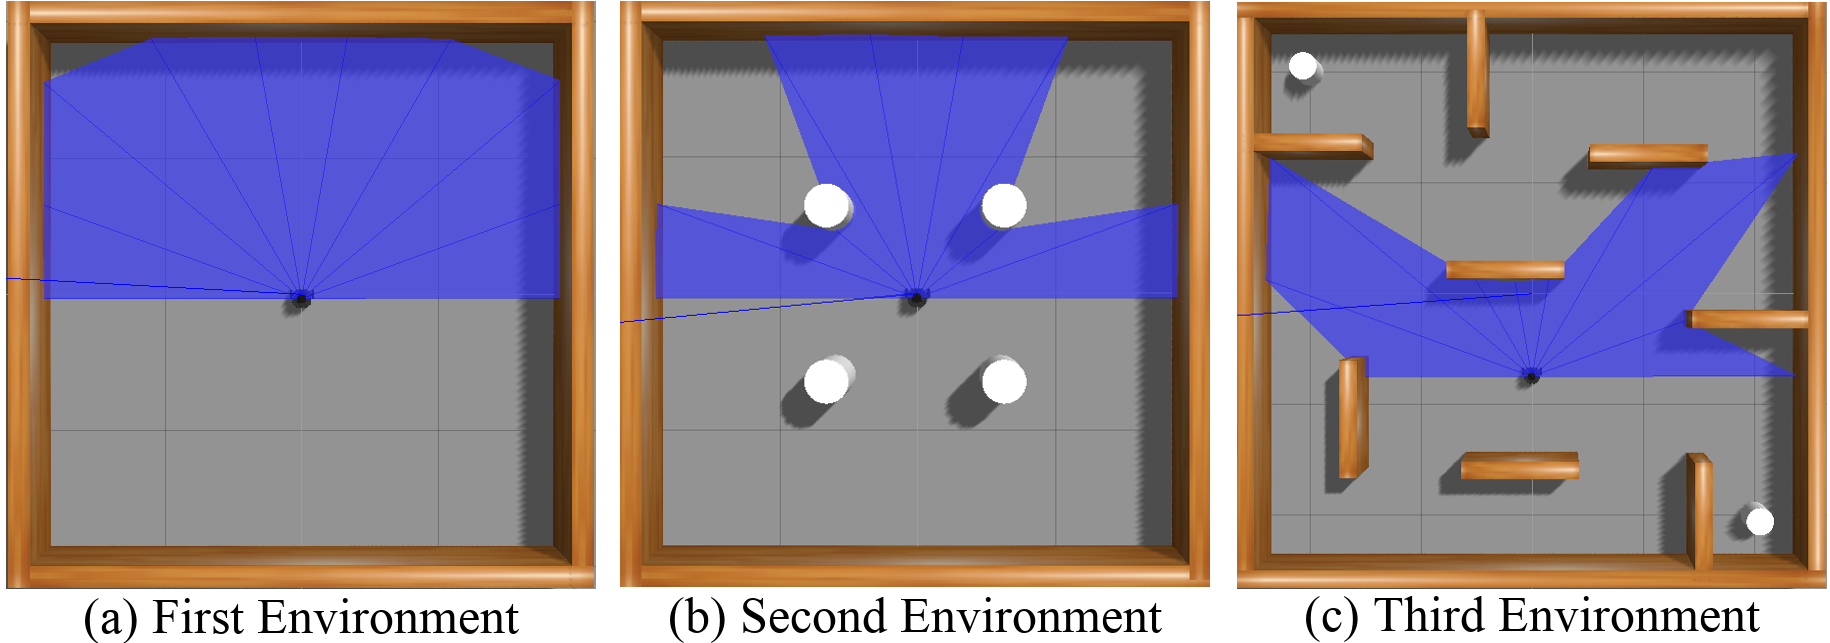
\includegraphics[width=\columnwidth]{images/environments1.png}}
\caption{Training environments used on Gazebo simulation. First environment (a), second environment (b) and third environment (c).}
\label{fig:environments}
\end{figure}

\subsection*{Reward Function}

Once the environment have been defined it is possible to simulate a controlled mobile robot for a navigation task.
Now it is necessary to define the reward and penalty system to the Deep-RL network.
Remembering that the rewards and penalties are attributed numbers passed to the intelligent agent.
So, the network will make a feedforward and backpropagation step in order to learn the hyperparameters.

There are four different conditions for the reward system that presented better results for the problem's resolution and are the following:
\begin{equation}
r (s_t, a_t) = 
\begin{cases}
r_{arrive} \ \textrm{if} \ d_t < c_d
\\
r_{collide} \ \textrm{if}\ min_x < c_o
\\
c_{r1}(d_{t-1} - d_t) \ \textrm{if} \ (d_{t-1} - d_t) > 0
\\
c_{r2} \ \textrm{if} \ (d_{t-1} - d_t) \leq 0
\end{cases}
\end{equation}

If the robot gets to the target through threshold checking $c_d$, a positive reward $(r_{arrive})$ is given, but if the robot collides with an obstacle through a minimum range readings checking, a negative reward $(r_{collide})$ is given.
Both conditions are sufficient to end the training episode.
Otherwise, the reward is based on the distance difference from the target compared to the last time step $(d_{t-1} - d_t)$. 
If this difference is positive the reward given is the distance traveled multiplied by the hyperparameter $(c_{r1})$, and if the distance is negative is used the hyperparameter $(c_{r2})$.
This motivates the mobile robot to get closer to the target position and encourages it to avoid the obstacles in the environment.

\subsection*{Positioning capture in real environments}

After the DDPG network training through simulation, it will be tested how effective can be a this type of network in a real environment.
A TurtleBot3, version Burger, will be used to perform this test. But for it is necessary to obtain the angle and distance of a target for the network to complete its goal. So it was setup a camera in the ceiling to extract this information.

Firstly, the essential points positions to extract the angle and distance are taken from the image.
These positions include the target, left and right side of the robot, and three points to be a distance reference parameter.
In Fig. \ref{fig:pixel_to_meter} is shown that were used different colored circles to identify the relevant points.
The yellow circle was attached to the target, the blue to the left side of the robot, the red to the right side and the three green circles were used by a reference parameter to calculate the distance.

\begin{figure}[H]
\centerline{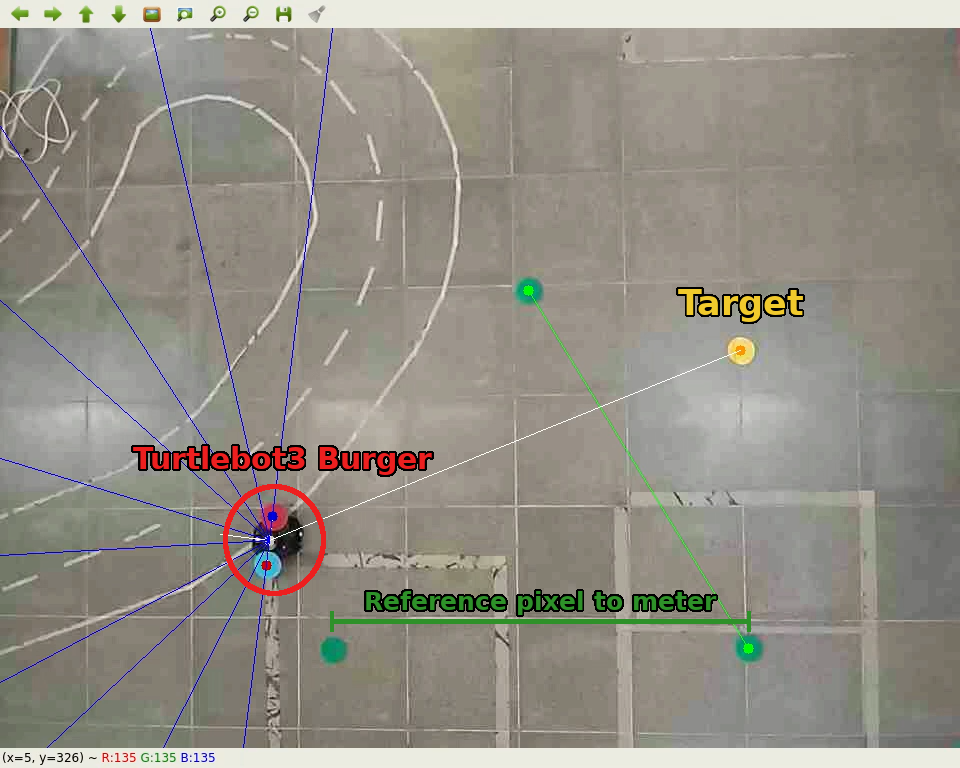
\includegraphics[width=10cm]{images/pixel_to_meter.png}}
\caption{Real environment relevant points}
\label{fig:pixel_to_meter}
\end{figure}


After the points were extracted from the center of the circles, it is possible to calculate the two necessary DDPG network inputs.
So, it is necessary to figure out the vector $distance$ that connects the center of TurtleBot3 to the target point, and the vector $direction$ which represents the direction of robot.
The vector $direction$ starts from the center of TurtleBot3, which is equal to the midpoint of the blue and red points.
The blue and red circles are on left and right sides of the mobile robot, respectively.
With this it possible to determine front of the robot.
%aqui vou escrever mais 
The center of green circles have a predefined distance from each other, what permits the calculation of robot and target distance by converting the pixel distance of the image to the distance in meters.
%aqui tbm




% e aeee
%acabei de perder meia hora no face AAAAAAA
% cara, na escrita n me dou mt bem, mas vou escrevendo o q vem na cabeça e após a gente estrutura melho
% faz isso mesmo meu KKKK eu sou meio travado na vdd mas to tentando (bem travado)
% a ideia é meter o louco e escrever tudo que vem na mente
% isso vem com a pratica SAUHSUAS, 
% pode se sentir a vontade pra mudar as coisas.
% só modifiquei pq achei melhor - ficou melhor assim msm ;)
% o que tu conseguir escrever eu e o professor gamarra corrigimos depois


%qual tu pensa a imagem pra colocar nessa subsection ae
%um frame com o alvo indicado, pixel meter parameter tb, e o robo? q nem o video do face? ---> meu acho que pode ser só uma imagem que contenha o robo, a referencia e tals (pode ser do primeiro ambiente que a gente tinha feito) ai tu explica através dela - OK

%coloquei a imagem do grafico com os obstáculos no drive, acho q ficou ok ---> eu vi, tá top na real - :D
% amanhã vou pegar pra escrever nos resultados, tava editando o modelo mais hj - azulzinho topi --> e as imagens pra ficarem melhor tbm
% vou pegar pra dormir aqui na real, flws o/// falooooow veéeei até amanhã


\section*{Results}

This section deals with the presentation and discussion of results.
The collected data are related to the obtained reward from the artificial neural network of the project.
With these data is possible to see what is the learning degree of the agent in the environment because the gained reward is intrinsically attached to the performance of the agent on the environment that it must go.
All the training environments were arranged by ROBOTIS, however, some alterations were done on the source code of the Gazebo simulation in order for the simulated mobile robot to use the reward system defined on this paper.

A mobile robot with a DDPG network was trained in order to make the experiments in the environments presented on Fig. \ref{fig:environments}, where the goal of the mobile robot is to get to the target.
For the first test was used the first environment that shows, in Fig. \ref{fig:amb1target}, a sequence of frames of the robot and the target. We can observe how the robot start in an initial position distant from the target, navigating in order to reach the target.

\begin{figure}[H]
\centerline{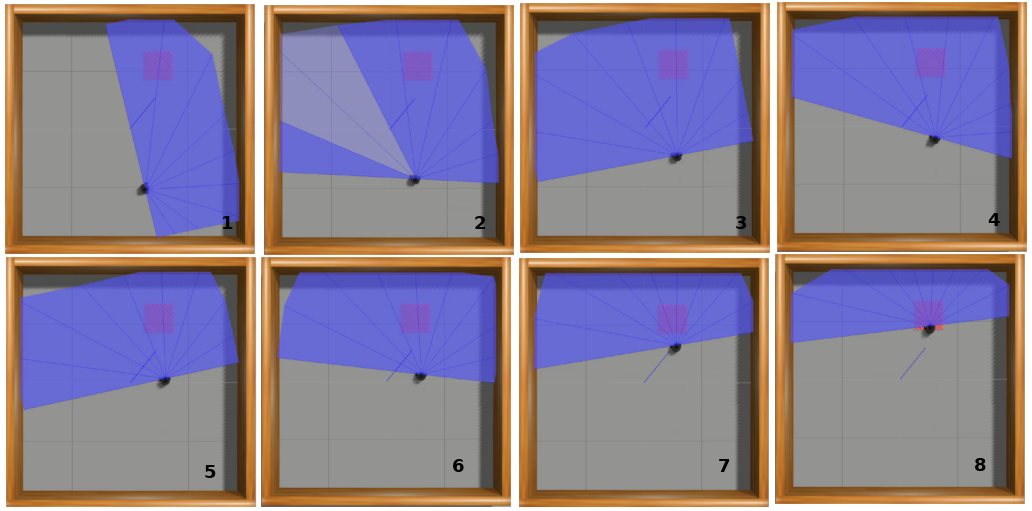
\includegraphics[width=\columnwidth]{images/amb1target.png}}
\caption{Images sequence in the first environment.}
\label{fig:amb1target}
\end{figure}

The training results of the reward function of the first environment are shown in Fig. \ref{fig:stage_1}.
On the first episodes can be noticed a negative reward, this happens because the algorithm started and it was still learning. 
This reward by episode means that the robot is trying to maximize the reward to complete the task. 
It is observed in the episode 400 a fall. 
This is a probable correction on some maximized parameters of the network and it resulted in a low reward.
Results like this means that the network has a continuous learning trying to correct itself. 

\begin{figure}[H]
\centerline{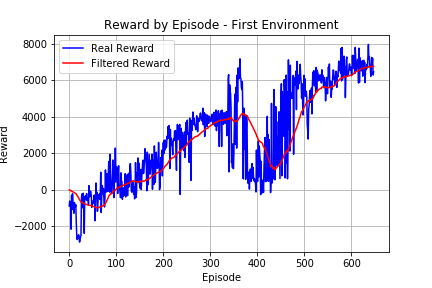
\includegraphics[width=10cm]{images/stage_1.png}}
\caption{Rewards of the first environment.}
\label{fig:stage_1}
\end{figure}

In Fig. \ref{fig:stage_1} the $x$ axis represents the past episodes on the simulation, an episode is defined when the mobile robot arrives to the target in the map or collides with some obstacle. 
The $y$ axis in Fig. \ref{fig:stage_1} represents the total value of the reward that the robot received on the episode.
The reward, with the blue color, has a great variance, it was decided to use a moving average filter for better visualization of the results.

After the mobile robot has been trained on the first environment, the experiment was done in the second environment and tested. It is shown in Fig. \ref{fig:amb2target} a sequence of the actions made by the TurtleBot from an initial position until it could arrive to the target after the training episodes.

\begin{figure}[H]
\centerline{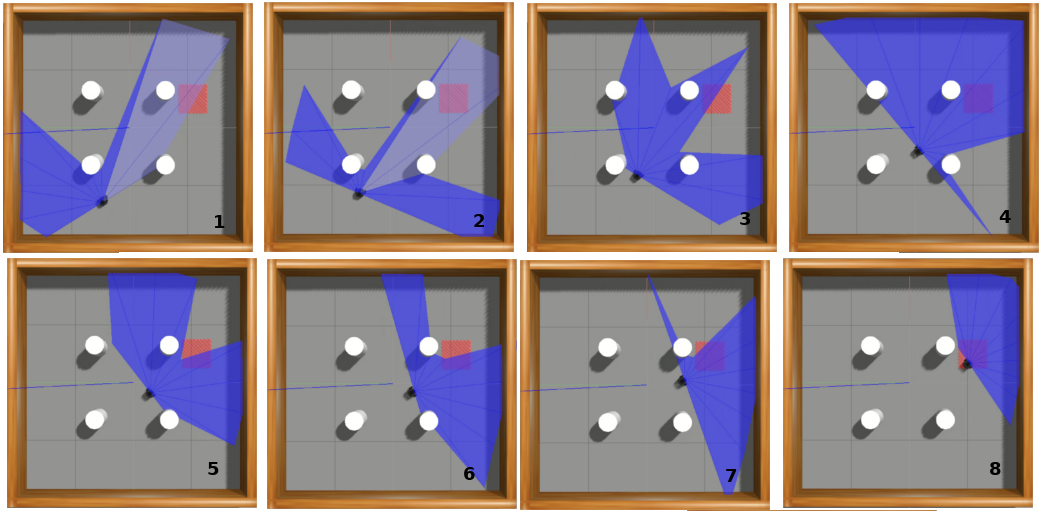
\includegraphics[width=\columnwidth]{images/amb2target.png}}
\caption{Images sequence in the second environment.}
\label{fig:amb2target}
\end{figure}

The reward function results of the training process for the second environment are shown in Fig. \ref{fig:stage_2}.
Comparing this results with the last environment, we can observe that it needed more episodes so the robot could present good results.
It is noticed that with a more complex environment, exists the possibility that an agent could take a longer time to get a good performance.

\begin{figure}[H]
\centerline{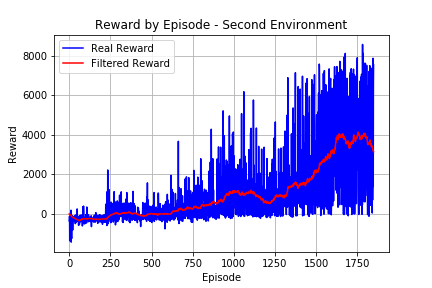
\includegraphics[width=10cm]{images/stage_2.png}}
\caption{Rewards of the second environment.}
\label{fig:stage_2}
\end{figure}

For the final test and the sequence of the actions made by the TurtleBot to arrive to the target after the training process it was used the third environment.  A sequence of the actions made by the TurtleBot to arrive to the target after the training episodes are shown in Fig. \ref{fig:amb3target}.

\begin{figure}[H]
\centerline{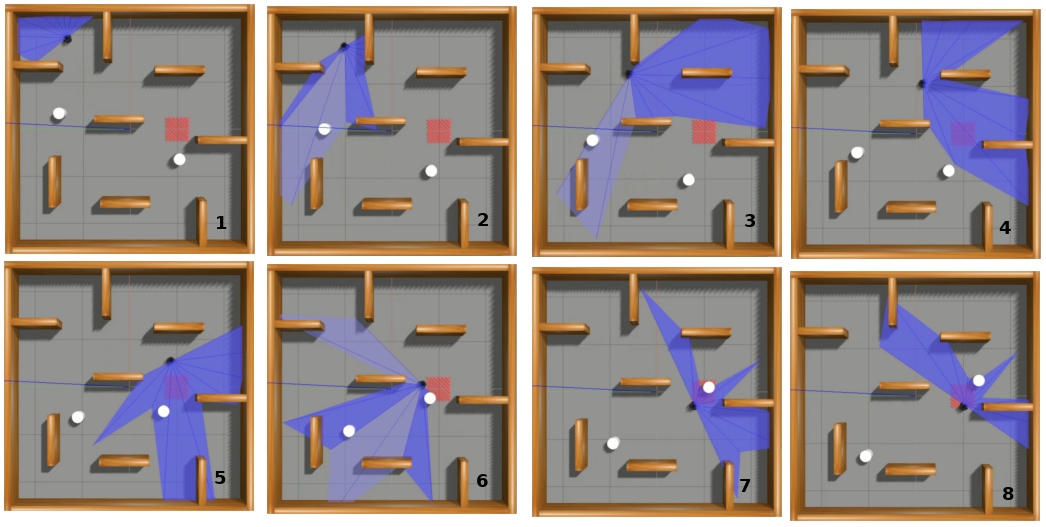
\includegraphics[width=\columnwidth]{images/amb3target.png}}
\caption{Images sequence in the third environment.}
\label{fig:amb3target}
\end{figure}

The results of the reward function of the last training environment is shown in Fig. \ref{fig:stage_4}.
On this environment, due to the high complexity, it was necessary a higher number of training episodes.
If compared the reward function with the previous Fig. \ref{fig:stage_1} and Fig. \ref{fig:stage_2}, it is possible to notice an average reward bellow two thousand.
This happens because to reach the target, which has the highest reward possible on comparison with the others, it is necessary that the agent could execute actions that do not generate too many points, however, that still makes it to arrive to the target.
Nevertheless, it was noticed by simulating the trained robot some actions that caused it to collide.
Many of these collisions were due to the moving dynamic obstacle close to the target.
This resulted in the agent making the decision of that mobile robot would collide or would try to avoid the obstacle.
The occurred behavior may have been caused because of the system created.
In order to resolve these actions, probably, it would be necessary to create a reward system that could bypass the error of the network.

\begin{figure}[H]
\centerline{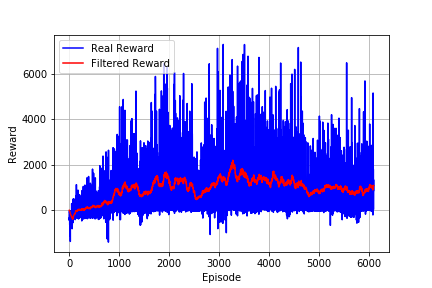
\includegraphics[width=10cm]{images/stage_4.png}}
\caption{Rewards of the third environment.}
\label{fig:stage_4}
\end{figure}

% Continua

After the training and validation of each simulation environment, it was created two more environments for the testing of the DDPG network in the real world.
The first real environment is shown in Fig. \ref{fig:real_envs} (a) and resembles the first simulation with no obstacles. The second environment is shown in Fig. \ref{fig:real_envs} (b) and it presents a complex environment similar to the second and third used on simulation with the exception of not having moving obstacles.

\begin{figure}[H]
\centerline{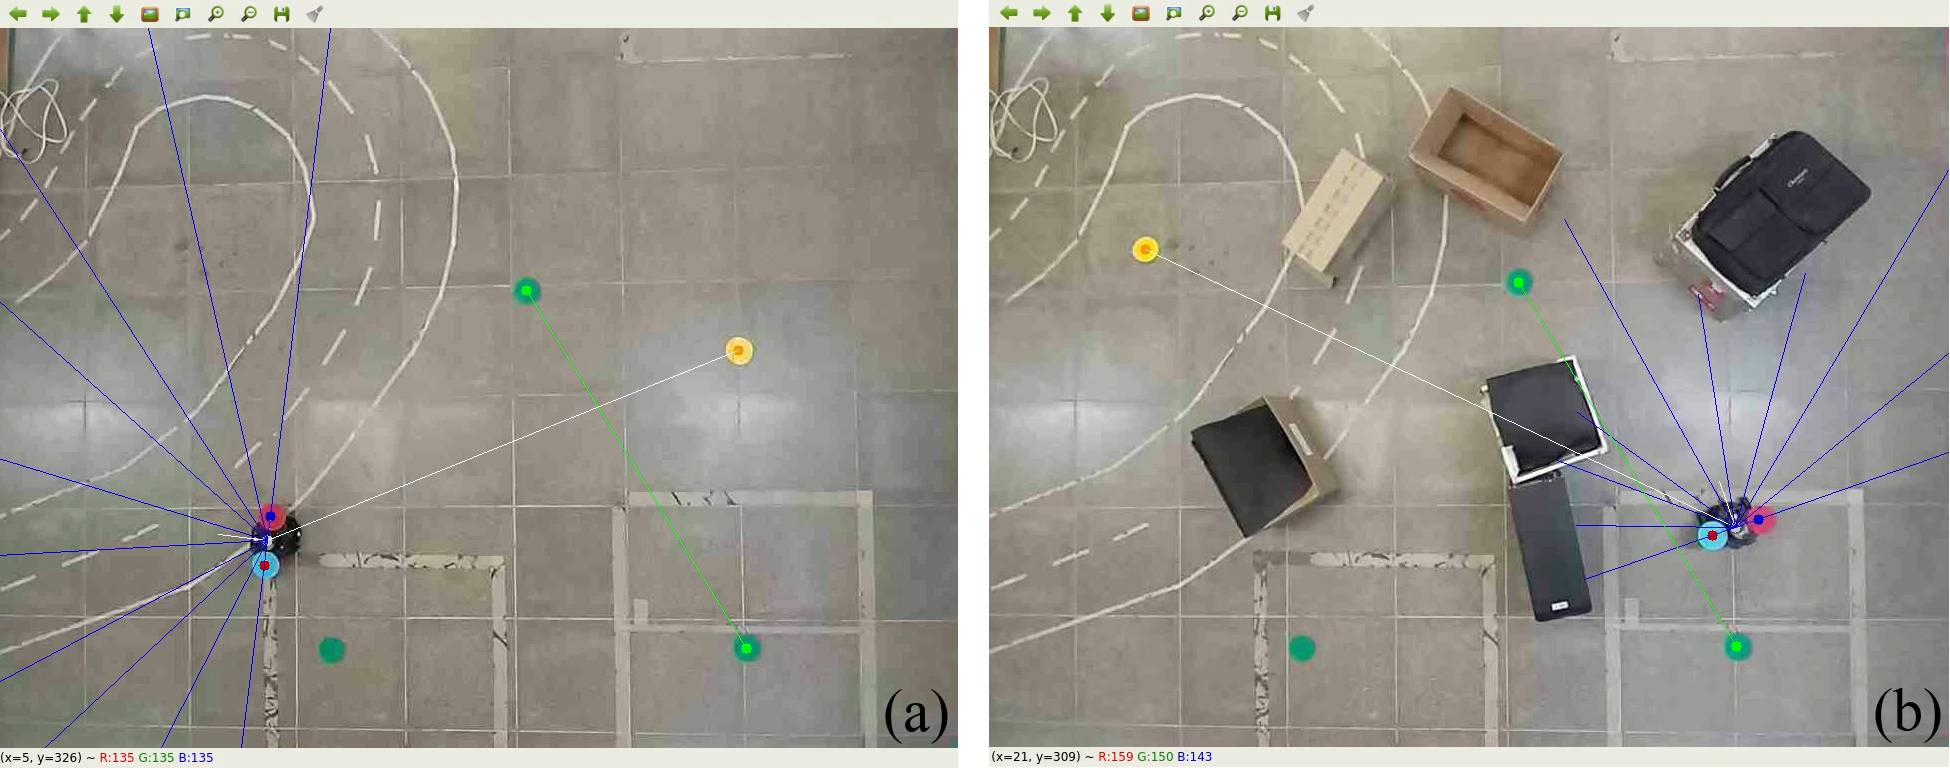
\includegraphics[width=12cm]{images/real_envs.png}}
\caption{Environments created for the DDPG test on the real world. First environment (a) and second environment(b).}
\label{fig:real_envs}
\end{figure}

With the target defined on the first real environment, it was executed the DDPG network on the Turtlebot3.
In the graph, shown in Fig. \ref{fig:env1_graph}, is possible to see the trajectory made by the network to arrive to the target.
In the Fig. \ref{fig:frames_env1} is shown by frames the trajectory made my the robot to complete the task.

\begin{figure}[H]
\centerline{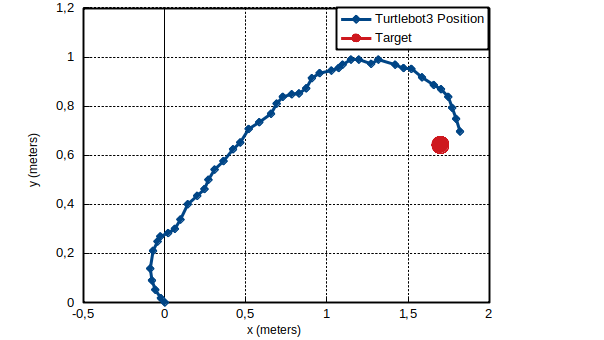
\includegraphics[width=12cm]{images/env1_graph.png}}
\caption{Trajectory of the Turtlebot3 in the first real environment}
\label{fig:env1_graph}
\end{figure}

\begin{figure}[H]
\centerline{\includegraphics[width=\columnwidth]{images/frames_env1.png}}
\caption{Images sequence of the Turtlebot3 in the first real environment}
\label{fig:frames_env1}
\end{figure}

For final test of the network, it was used the second real environment. In the graph, shown in Fig. \ref{fig:env2_graph}, even with obstacle the network was capable to arrive to the target. In the Fig. \ref{fig:frames_env2} is shown by frames the trajectory made my the robot to complete the task. %So, with these results applied on real world environment we can see how effective can be a DDPG network trained in simulation environment
The robot was able to accomplish both task given in the real world environments.
This shows how effective can be the DDPG networks, trained in a simulation environment, in completing complex tasks on physical environment.

\begin{figure}[H]
\centerline{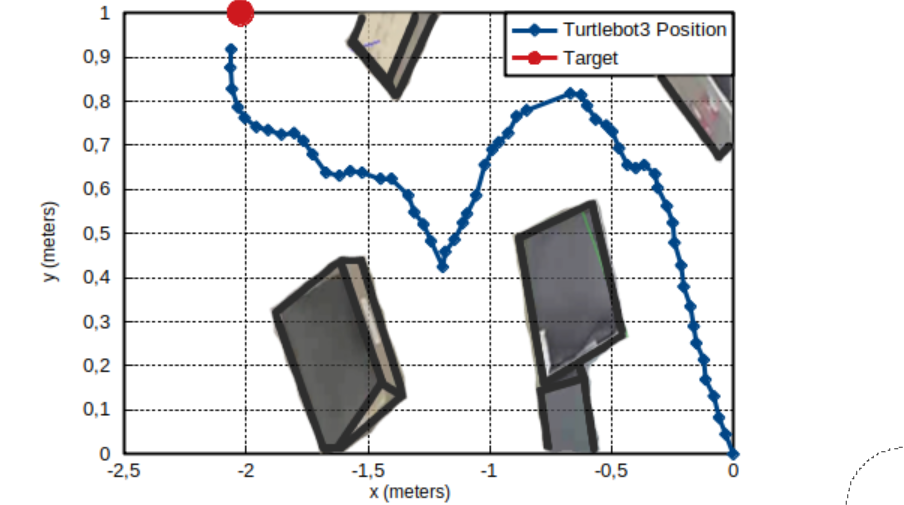
\includegraphics[width=12cm]{images/env2_graph.png}}
\caption{Trajectory of the Turtlebot3 in the second real environment}
\label{fig:env2_graph}
\end{figure}

\begin{figure}[H]
\centerline{\includegraphics[width=\columnwidth]{images/frames_env2.png}}
\caption{Images sequence of the Turtlebot3 in the second real environment}
\label{fig:frames_env2}
\end{figure}

\section*{Conclusion}

In this paper was developed a neural network, DDPG, to be used on navigation of a mobile robot through continuous control in a virtual environment.
Thus achieving a deep reinforcement learning network structure able to solve the problem of robot navigation.
It was proposed as a task that the robot could reach a target position in different simulated environments and it created a reward function so that the DDPG network could give as results, the linear and angular velocity for the robot. All the network structure created was applied on the Gazebo simulation environments with success.

With the training results obtained on the simulation environments, it was analyzed the performance of the intelligent agent algorithm in the task of avoiding obstacles and getting to the final goal. 
On the three environments proposed, the algorithm had a good performance, however, in the last environment it was observed that sometimes even after many training episodes the mobile robot would still collide with some obstacle.

It is possible to conclude that DDPG networks are suitable for the development of applications that need a continuous control on the robotics.
The Deep-RL networks can produce excellent results if the reward system is well-made for the problem that it wants to solve.
It was proved that intelligent agents can move around in a complex simulated environments as well as in real world environments without any previous knowledge of the environment.
The network based on deep deterministic policy gradients can provide means of unifying the machine learning for the control of robotic systems.
This technique can be applied in function as manipulation of robotic arms, pendulums, games among others.
% As future works, it is intended to use the deep reinforcement learning technique for the navigation of the TurtleBot3 Burger robot in a real environment, thus, being able to validate the training in a simulated environment in a real environment.

\bibliographystyle{apacite}
\bibliography{bib}

\end{document}
